\documentclass[11pt]{article}
% ACL requires \documentclass to be the first line, so \pdfoutput follows it;
% arXiv only needs the directive within the first few lines. FHA-443 — NLLP 2026
% submission, ACL two-column format, review mode.
\pdfoutput=1
\usepackage[review]{acl}
\usepackage{times}
\usepackage{latexsym}
\usepackage[T1]{fontenc}
\usepackage[utf8]{inputenc}
\usepackage{microtype}
\usepackage{inconsolata}
\usepackage{graphicx}
\usepackage{float}
\usepackage{amsmath}
\usepackage{booktabs}
\usepackage{makecell}
\usepackage{xurl}

% article's twocolumn mode sets \flushbottom, which pads a short column to full
% depth by stretching the rubber glue around display math and floats; in a paper
% this float-heavy that reads as inch-high gaps above figures.
\raggedbottom

\title{FHA-443: An Evidence-Anchored Corpus and Extractor for \\ Fair Housing Act Doctrine in U.S.\ District-Court Opinions}

\author{Anonymous NLLP submission}

% Line numbers come from acl.sty's [review] option unchanged: each column's
% ruler sits in the page margin on that column's outer edge at 8pt, so neither
% enters the 0.6cm gutter. check_rulers.py verifies that on every page.

% Where the artifact lives, written once. Under [review] the paper points at the
% anonymous supplement; \usepackage[final]{acl} reveals the repository without a
% second edit, so the URL cannot be left out of the camera-ready by accident and
% cannot leak into the blind copy.
\makeatletter
\newcommand{\repowhere}{\ifacl@anonymize
\url{https://anonymous.4open.science/r/fha-federal-courts-7B74/README.md}\else
\url{https://github.com/garyzhang1006/fha-federal-courts}\fi}
\makeatother

\begin{document}
\maketitle

\begin{abstract}
Fair Housing Act cases are decided overwhelmingly in federal district courts, but computational work has followed the appellate record, leaving no trial-court corpus. We release FHA-443: 757 canonicalized Nature of Suit 443 district-court opinion clusters, 751 with full text and 417 rule-positive and substantive. An evidence-anchored extractor labels five doctrinal constructs and the proof framework and attaches character-offset snippets to its regex matches. We validate it against 93 blind hand-coded opinions and a frozen three-pass Claude Opus 4.8 baseline, 98.8\% unanimous across 1,215 claim decisions. Micro $F_1$ rises from 0.767 to 0.872 and framework accuracy from 0.774 to 0.914, with the largest gain in disparate impact. Rule-based disparate-impact detection reaches precision 0.41 because it fires on recitations, citations, and unreached claims; the frozen model labels reach precision 1.00 at unchanged recall. Refusal and steering defeat both extractors, at $F_1$ 0.67 and 0.61. The corrected labels overturn the raw reading of the docket: disparate treatment leads at 46.1\% against 13.2\% for disparate impact (exact McNemar $p<.0001$), and circuits diverge from 8\% to 54\% in impact language ($p<.001$), so any cross-circuit index must be case-mix adjusted. Corpus, extractor, codebook, and frozen labels are released at \repowhere.
\end{abstract}

\section{Introduction}

Almost every Fair Housing Act dispute that reaches a federal judge is resolved by a district court, and almost every computational study of the statute reads appellate opinions instead \citep{seicshnaydre2013}. No public corpus of district-court FHA opinions exists, so the basic descriptive question of which theories plaintiffs actually litigate has no measured answer.

Building one is a legal information-extraction problem with a specific failure mode. A district-court opinion recites the governing standard for every theory it discusses, cites cases applying theories it will not reach, and disposes of most claims on procedural grounds. A keyword rule cannot tell a recitation from an adjudication, and the confusion is asymmetric: disparate impact has a canonical three-step recitation that appears in opinions deciding nothing about impact, while reasonable accommodation is usually named only when it is at issue. An extractor here has to separate what an opinion mentions from what it decides, and expose the evidence so the error can be found.

We build that extractor and measure how far it gets. FHA-443 holds 757 canonicalized Nature of Suit 443 opinion clusters, 751 with full text and 417 rule-positive and substantive. A deterministic layer labels five doctrinal constructs and the proof framework, attaching character offsets and snippets to its matches, and a frozen three-pass Claude Opus 4.8 baseline given the same codebook provides the comparison. Against 93 blind hand-coded opinions the model route is better on every aggregate measure, with the largest gain in disparate impact. Rule-based disparate-impact detection runs at precision 0.41 for exactly the reason above, while the frozen model labels reach 1.00 without costing recall. Refusal and steering defeat both routes, which we read as heterogeneity in how courts describe the conduct rather than a limit of either method.

Correcting the labels changes what the docket looks like. The rule system makes the three leading theories appear within ten points of one another. On a fresh random draw scored by the baseline, disparate treatment leads at 46.1\% against 22.4\% for accommodation and 13.2\% for impact, and the lead survives an exact McNemar test on paired within-case labels. Circuits split on the doctrine they apply, from 8\% impact language in the Tenth to 54\% in the Seventh, so a cross-circuit comparison that ignores case mix reports docket composition as enforcement.

The reason to measure this signal is that residential segregation has outlasted the legal barriers that produced it, and the Fair Housing Act is the principal federal instrument aimed at it \citep{fha1968,schelling1971}. Whether the signal courts emit moves where people live is the question behind the corpus, and this paper cannot answer it: the legal and housing series overlap in one year, yielding eight matched cells and no within-unit variation. We report that boundary as a result, and in its place state the behavioral condition under which such a signal could move sorting at all (Appendix~\ref{app:scoping}).

The paper contributes three things. First, FHA-443, the first public corpus of federal district-court FHA opinions, with an evidence-anchored multi-label schema for proof theory, duty, conduct, framework, remedy, and outcome cues. Second, a validation of that schema against blind human coding and a frozen LLM baseline that locates the failure precisely, at disparate-impact precision under rule-based extraction and at refusal or steering under both. Third, a corrected description of the trial docket, treatment-led rather than flat, together with a measured circuit split that makes case-mix adjustment a requirement for any index built on this text.

\section{Related Work}

This work sits in the computational-social-science tradition that treats segregation as an emergent outcome of local rules, for which Schelling's dynamic model is the canonical account \citep{schelling1971} and the Black--White dissimilarity index the standard measure \citep{massey1988}. Our contribution measures the legal signal and uses a separate scoping model to state one possible channel into that mechanism.

On measurement we follow the text-as-data program, which recovers social quantities from large corpora while warning about selection, measurement error, and researcher-defined dictionaries \citep{grimmer2013}. Legal natural language processing supplies capable representations of judicial text \citep{chalkidis2019,chalkidis2020,guha2023}, but prediction accuracy and construct measurement are different goals. Recent work at this workshop reports the gap directly. Large models remain unstable and poorly calibrated to human interpretive judgments \citep{purushothama2025}, they underperform a domain-pretrained encoder on fine-grained legal argument types \citep{held2025}, and automated statute consolidation reaches high textual similarity while leaving legally significant errors \citep{prior2025}. Work that links platform policy text to enforcement decisions makes the same design choice we make, building a human gold standard and reporting where the automated link fails \citep{esser2025}. We therefore give every headline indicator a rule and an evidence offset, and cross-check it against a stronger extractor rather than trusting either route alone.

On the legal side, appellate work documents variation in Fair Housing Act disparate-impact claims \citep{seicshnaydre2013}, and empirical-legal scholarship stresses the difficulty of causal inference in selected litigation \citep{ho2011,priest1984}. Litigated opinions are a selected sample of disputes, so we treat our shares as measurements of a defined retrieval, not of all housing conflict. Two gaps follow. No public corpus of federal district-court Fair Housing Act opinions exists, so the trial-level composition of asserted theories has never been measured. And no prior work sets this measured legal-enforcement signal beside a Schelling access mechanism. This paper closes the first and scopes the second without estimating a link between them.

\section{Data}

We build the corpus from CourtListener, the open-access case-law database maintained by the Free Law Project \citep{freelaw2024}. We freeze a bulk-derived snapshot because API quotas and changing metadata give no stable route to the complete corpus. Every retained observation is a federal district-court opinion, and the archive preserves raw candidate and exclusion files alongside normalized fields, so a reader can distinguish a source record, a canonical cluster, and a rule-positive observation.

We imported the opinion bulk dump into PostgreSQL, preserved source HTML, and mapped court identifiers to circuits with a hand-verified crosswalk, making the circuit a geographic aggregation key. We exclude the D.C.\ Circuit, which covers only the District of Columbia and hears mostly federal agency rather than regional housing cases, so it does not function as a geographic unit for the segregation linkage. The metadata pass produced 937 candidate rows, and exact NOS normalization retained 757 official or unambiguous NOS-443 rows, all district-court observations. Opinion volume concentrates in recent years (Figure~\ref{fig:volume}).

\begin{figure}[H]
\centering
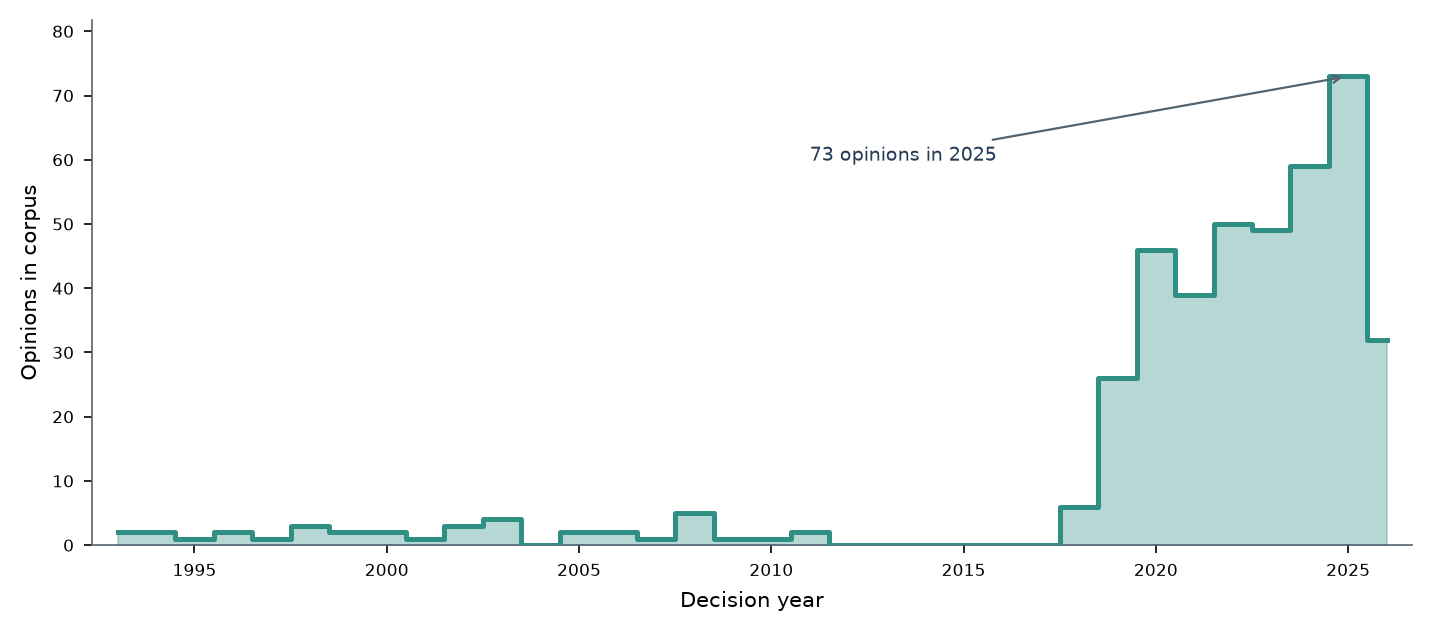
\includegraphics[width=\columnwidth]{media/image5.png}
\caption{Federal FHA opinion volume concentrates in recent years.}
\label{fig:volume}
\end{figure}

Because NOS coding is a docketing convention rather than a merits label, canonical cases can mix incidental references with FHA decisions, and citations may appear in procedural history. The rule therefore requires 200 characters, exact NOS-443 normalization, and either a core citation or an Act-name match. Equation~\ref{eq:inclusion} is a high-recall selection frame within the retrieval; writing $L_i$ for text length, $N_i$ for the NOS code, $C_i$ for a core FHA citation, and $A_i$ for an Act-name match,
\begin{equation}\label{eq:inclusion}
I_i = \mathbf{1}\{L_i \ge 200\}\cdot\mathbf{1}\{N_i = 443\}\cdot\mathbf{1}\{C_i \lor A_i\}
\end{equation}
Hand-coded validation evaluates downstream indicators, so 417 is a rule-positive denominator.

Full text is recovered for 751 of 757 canonical clusters (99\%), and the remaining six lack retrievable text. The 757 retained records and 180 excluded candidates in the repository reconstruct the 937-row candidate set, so the retained sample is this CourtListener district-court retrieval. The representativeness comparison concerns retrieval composition only. Section~\ref{sec:validation} and Table~\ref{tab:gold} report the hand-coded set and the construct-specific accuracy it supports.

\section{Methods}

\subsection{Structured legal-variable extraction}\label{sec:extraction}

The task is multi-label classification over a full opinion with inspectable rule matches. The input is the text of one district-court opinion cluster. The output is a record with six binary construct labels, disparate treatment, disparate impact, refusal or steering, reasonable accommodation, exclusionary zoning, and an outcome cue, one categorical proof-framework label, and character spans with the passages that triggered deterministic matches. Labels are nonexclusive, because an opinion can adjudicate a duty and a course of conduct at once. A span does not itself separate recitation from application; it exposes the match so a reader can find that error rather than relying only on a second annotator.

From each opinion, deterministic regex and lexicon rules create a structured legal record (Appendix~\ref{app:pipeline}). Each label names a doctrine, and the doctrine fixes what counts as a positive. Disparate treatment is intentional differential handling of a housing transaction, and at the trial level it is usually litigated through the burden-shifting structure of \citet{mcdonnell1973}. Disparate impact reaches a facially neutral practice through its effects, on the logic of \citet{griggs1971}, recognized under the Fair Housing Act in \citet{inclusive2015} and implemented by HUD in 2013 \citep{hud2013} and 2023 \citep{hud2023}. Reasonable accommodation is the disability-related duty in 42 U.S.C.\ \S~3604(f)(3)(B) \citep{fha1968}, so it can co-occur with either theory. Refusal or steering and exclusionary zoning describe conduct, by a private actor and by a municipality. The labels sit at three levels, proof, duty, and conduct, and the schema keeps them separate rather than forcing one winner per opinion. Stored spans let readers audit whether a matched passage applies a doctrine or only recites it, a live instance of the gap between the law as written and the law as applied \citep{pound1910}.

Snippets and character offsets support every flag, including an archived ``summary judgment'' match at offsets 1613--1629. We retain a negation-sensitive alternative for sensitivity analysis, while the headline run uses the unscoped rule. Outcome evidence is separate, and the outcome cue is null when cues are mixed or absent. Because the rules are deterministic, a reader can identify a false positive, revise a rule, and recompute the measure.

\subsection{The enforcement index}

We aggregate opinion-cluster measurements to circuit-year cells to form the Federal Enforcement Intensity Index, an equal-weight composite of log opinion volume, a shrunk directional outcome-cue rate, and normalized remedy-cue intensity. Doctrinal breadth stays outside the composite. Appendix~\ref{app:feii} gives the definition, the shrinkage constant, and the reason we do not fit weights.

\subsection{External-data feasibility boundary}\label{sec:feasibility}

We attempted to link circuit enforcement to residential segregation. The outcome is county Black--White dissimilarity \citep{massey1988} computed from ACS tract counts \citep{census2022} and population-weighted to circuit geography, with HMDA denial rates \citep{cfpb2024} as a complementary measure. Legal and housing coverage overlap in a single year, which yields eight matched 2022 cells and no within-unit variation. We therefore report the merge as a feasibility result and defer identification to a later design, since one observed year cannot separate a legal signal from stable circuit characteristics or national conditions.

\subsection{Validating against hand coding}\label{sec:validation}

We hand-coded 120 candidate opinions blind to machine labels, including machine-flagged holdings and a claim-by-era sample, so the overlap is enriched rather than random. After exact NOS-443 normalization, 93 opinions overlap the canonical corpus and all 30 second-pass cases remain. We report construct-specific precision, recall, $F_1$, and $\kappa$ as diagnostic rates on that sample, not corpus-wide error rates.

\begin{table}[t]
\centering\small
\begin{tabular}{lcccc}
\toprule
\textbf{Variable} & \textbf{P} & \textbf{R} & $\mathbf{F_1}$ & $\boldsymbol{\kappa}$ \\
\midrule
\input{../outputs/paper_tables/table1_gold_rows.tex}
\end{tabular}
\caption{Diagnostic extraction accuracy on the 93-case enriched, choice-based canonical-corpus overlap. Human coding is the reference; 30 cases carry a second pass; metrics are not population weighted; the micro-average pools decisions rather than averaging rows.}
\label{tab:gold}
\end{table}

Accuracy varies across constructs (Table~\ref{tab:gold}). Disparate-impact detection recovers 0.92 of hand-coded positives at precision 0.41, so its $F_1$ of 0.56 suits screening while its false-positive rate limits direct prevalence claims. Framework accuracy is 0.77 ($\kappa=0.47$), holding-cue detection is 0.71/0.59/0.64, and binary agreement on 37 decisive cases is 0.81 ($\kappa=0.61$). Framework accuracy treats a single-framework prediction as compatible with a human \texttt{both} label; framework $\kappa$ excludes that case and is computed on the remaining four-class labels. The 30 double-coded cases show claim $\kappa=0.90$, framework $\kappa=0.86$, and four-way-winner $\kappa=0.73$.

Negation scoping shifts headline shares by at most 2.40 points (Appendix~\ref{app:negation}); writing $\theta_j$ for the share of construct $j$,
\begin{equation}\label{eq:negation}
\Delta_j = \theta_j^{\text{scope}} - \theta_j^{\text{headline}}
\end{equation}
micro precision, recall, and $F_1$ become 0.76, 0.75, and 0.76, and the treatment--impact ordering survives.

\subsection{LLM baseline and error correction}\label{sec:llm}

To test regex and lexicon behavior against a stronger extractor, we froze a Claude Opus 4.8 comparison. The model was instructed with the released codebook and returned the five claim labels and the framework field in three independent passes. Writing $y^{(p)}_{ij}$ for the label pass $p$ assigns and $\mathcal{D}$ for the set of scored opinion--construct cells, the reported label is the majority and the reported stability is the share of cells on which the passes never disagree:
\begin{align}
\tilde{y}_{ij} &= \mathbf{1}\Big\{\textstyle\sum_{p=1}^{3} y^{(p)}_{ij} > \tfrac{3}{2}\Big\},\label{eq:vote}\\
U &= \frac{1}{|\mathcal{D}|}\sum_{(i,j)\in\mathcal{D}}\mathbf{1}\big\{\big|\{y^{(p)}_{ij}\}_{p\le 3}\big| = 1\big\}.\label{eq:unanimity}
\end{align} The released scoring artifact retains those labels but not raw responses or claim-level evidence quotations, so the offline workflow reproduces scoring from frozen outputs rather than model inference. Across the 1,215 claim decisions on the overlap and draw, 98.8\% were unanimous. That figure records sampling stability under one model run, not agreement between independent coders. The run covers the 93-case human overlap and a uniform 150-case draw, seeded 20260720, from the 658 clusters outside the human set. Of 729 requested passes, 728 returned, and the single two-pass case agreed on all six fields. One model at one setting measures what Opus 4.8 recovers, not a property of LLM extraction. Opus 4.8 was the current Opus model when the labeling was performed, and Opus 5 was released afterward; a 20-case replication of the identical protocol with Opus 5 agrees with the frozen labels on 99 of 100 claim decisions, at micro $F_1$ 0.845 against 0.857 and disparate-impact precision 1.00 under both.

On the human overlap, LLM micro $F_1$ rises from 0.767 to 0.872 and framework accuracy from 0.774 to 0.914 (Table~\ref{tab:llm}). Disparate-impact precision rises from 0.407 to 1.000 at recall 0.917, and accommodation $F_1$ from 0.883 to 0.971. The rule detector fires on standard recitations, case citations, and claims the court does not reach; the frozen model labels remove those false positives at unchanged recall. Refusal or steering moves the other way, from $F_1$ 0.667 to 0.607, and is weak under both routes.

\begin{table}[H]
\centering\small
\setlength{\tabcolsep}{3.4pt}
\begin{tabular}{lccr}
\toprule
\textbf{Construct} & \textbf{Regex} & \textbf{LLM} & $\boldsymbol{\Delta F_1}$ \\
 & \scriptsize P/R/$F_1$ & \scriptsize P/R/$F_1$ & \\
\midrule
\input{../outputs/paper_tables/table2_llm_rows.tex}
\end{tabular}
\caption{Regex and LLM extraction diagnostics on the 93-case human overlap, per construct. Every row reproduces from \texttt{make reproduce} in the released repository.}
\label{tab:llm}
\end{table}

An open-weight replication places that gain in the extraction route rather than the model: qwen3:32b, given the same codebook and untruncated text, recovers impact precision 0.909 (Figure~\ref{fig:open}; Appendix~\ref{app:llmprotocol}). Its shortfall is asymmetric---58 false negatives against the frozen model's 19, but 11 false positives against 19---so the open model under-detects rather than disputing what counts as a claim.

\begin{figure}[H]
\centering
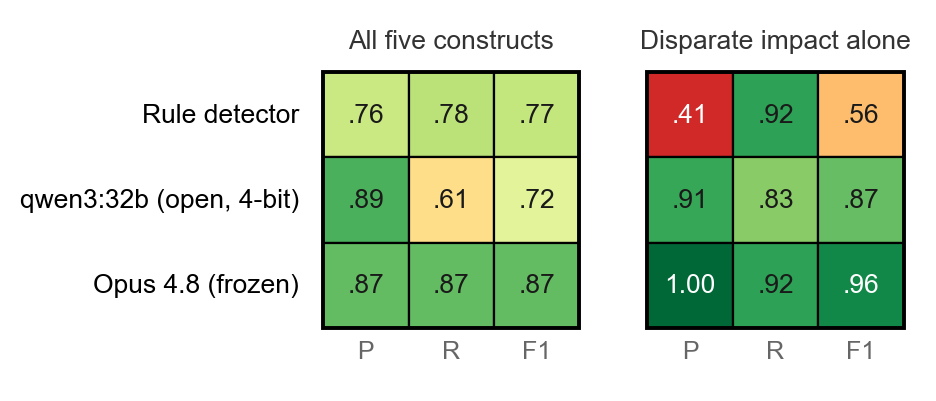
\includegraphics[width=\columnwidth]{media/image19.png}
\caption{Extraction diagnostics by route on the 93-case human overlap, shaded by value. The rule detector's disparate-impact precision is the only cell in the low band; both model routes recover it, and the open route pays for that precision in recall rather than in disagreement over what counts as a claim.}
\label{fig:open}
\end{figure}

The random draw contains 76 substantive cases. We compare its shares with the 417-case regex shares and a precision--recall correction. Where the overlap's precision $P_j$ and recall $R_j$ transport to the corpus, the rate of correct positives can be read off either margin, $\theta_j R_j = \Pr(\hat{y}_{ij}\!=\!1,\, y_{ij}\!=\!1) = \hat{\theta}_j P_j$, so the corrected share of construct $j$ is
\begin{equation}\label{eq:correction}
\theta_j = \hat{\theta}_j\,\frac{P_j}{R_j},
\end{equation}
clipped to $[0,1]$ in the implementation. Written this way the correction carries its assumption on its face: it is exact when the diagnostic rates transport and off by their drift when they do not. The draw provides a robustness check with model-generated labels, while calibration comes from the human overlap.

\section{Results}

\begin{table*}[t]
\centering\small
\setlength{\tabcolsep}{6pt}
\begin{tabular}{lll}
\toprule
\textbf{Sample (n)} & \textbf{Primary use} & \textbf{Does not license} \\
\midrule
\makecell[l]{Full-text\\corpus (751)} & \makecell[l]{Retrieval coverage,\\corpus construction} & \makecell[l]{Representative prevalence\\or causal claims} \\
\addlinespace[2pt]
\makecell[l]{Substantive\\clusters (417)} & \makecell[l]{Rule-defined\\prevalence, index} & \makecell[l]{Random-sample estimates\\or housing effects} \\
\addlinespace[2pt]
\makecell[l]{Random draw\\(150; 76 subst.)} & \makecell[l]{Frozen LLM prevalence,\\paired tests} & \makecell[l]{Human-gold accuracy or\\independent category tests} \\
\addlinespace[2pt]
\makecell[l]{Human overlap\\(93; 30 2nd pass)} & \makecell[l]{P, R, $F_1$, agreement\\diagnostics} & \makecell[l]{Corpus-wide error rates or\\untested transport} \\
\addlinespace[2pt]
\makecell[l]{Housing merge\\(8 cells; 2022)} & \makecell[l]{Data-availability,\\estimability check} & \makecell[l]{Index--sorting estimation\\or temporal inference} \\
\bottomrule
\end{tabular}
\caption{Analytic samples and inferential scope.}
\label{tab:samples}
\end{table*}

\subsection{The shape of the federal FHA docket}\label{sec:docket}

Table~\ref{tab:samples} maps the denominators used below. Across 417 substantive clusters, raw regex places disparate treatment first at 37.6\%, accommodation at 35.5\%, impact at 28.1\%, refusal or steering at 23.7\%, and zoning at 9.4\%. Indicators overlap, because accommodation records a duty while refusal and zoning describe conduct. The three leading shares fall within ten points of one another, so the docket appears near-flat. That flatness is an artifact of the impact detector's 0.41 precision, which inflates prevalence through standards, citations, and unreached claims.

The new baseline changes the substantive reading. In the 150-case draw, 76 clusters satisfy the substantive rule. The LLM majority identifies treatment in 46.1\%, accommodation in 22.4\%, impact in 13.2\%, refusal in 17.1\%, and zoning in 7.9\%. Treatment exceeds accommodation by 23.7 points (exact paired $p=.0096$) and impact by 32.9 points ($p<.0001$). Accommodation exceeds impact by 9.2 points ($p=.21$). These are two-sided exact McNemar tests on the same 76 cases, using discordant within-case pairs. Writing $b$ and $c$ for the two discordant counts and $d = b + c$, the reported value is an exact binomial tail rather than a $\chi^2$ approximation:
\begin{equation}\label{eq:mcnemar}
p = \min\Big(1,\ 2^{1-d}\!\!\sum_{k=0}^{\min(b,c)}\!\binom{d}{k}\Big).
\end{equation}
The test conditions on $d$, so only opinions where the two constructs disagree carry information; the 76 cases set how many such pairs exist, not the statistic itself, which is why a gap of 9.2 points can be directional and still unresolved. Labels are nonexclusive, so the tests compare paired prevalence, not independent category counts or causal effects. The treatment lead is significant. The accommodation-over-impact gap is directional but unpowered, at 23.6\% power at $n=76$. An exact-McNemar analysis places 80\% power at 295 substantive cases, about 583 total draws (Figure~\ref{fig:power}). The ordering may stay unresolved even then: the favour-accommodation share rests on 23 discordant pairs, its Wilson interval $[0.449, 0.812]$ includes 0.5, and averaging power over that uncertainty gives an assurance of only 0.64 at the nominally powered size. A human-coded random sample of that size would also replace the model-generated labels.

\begin{figure}[H]
\centering
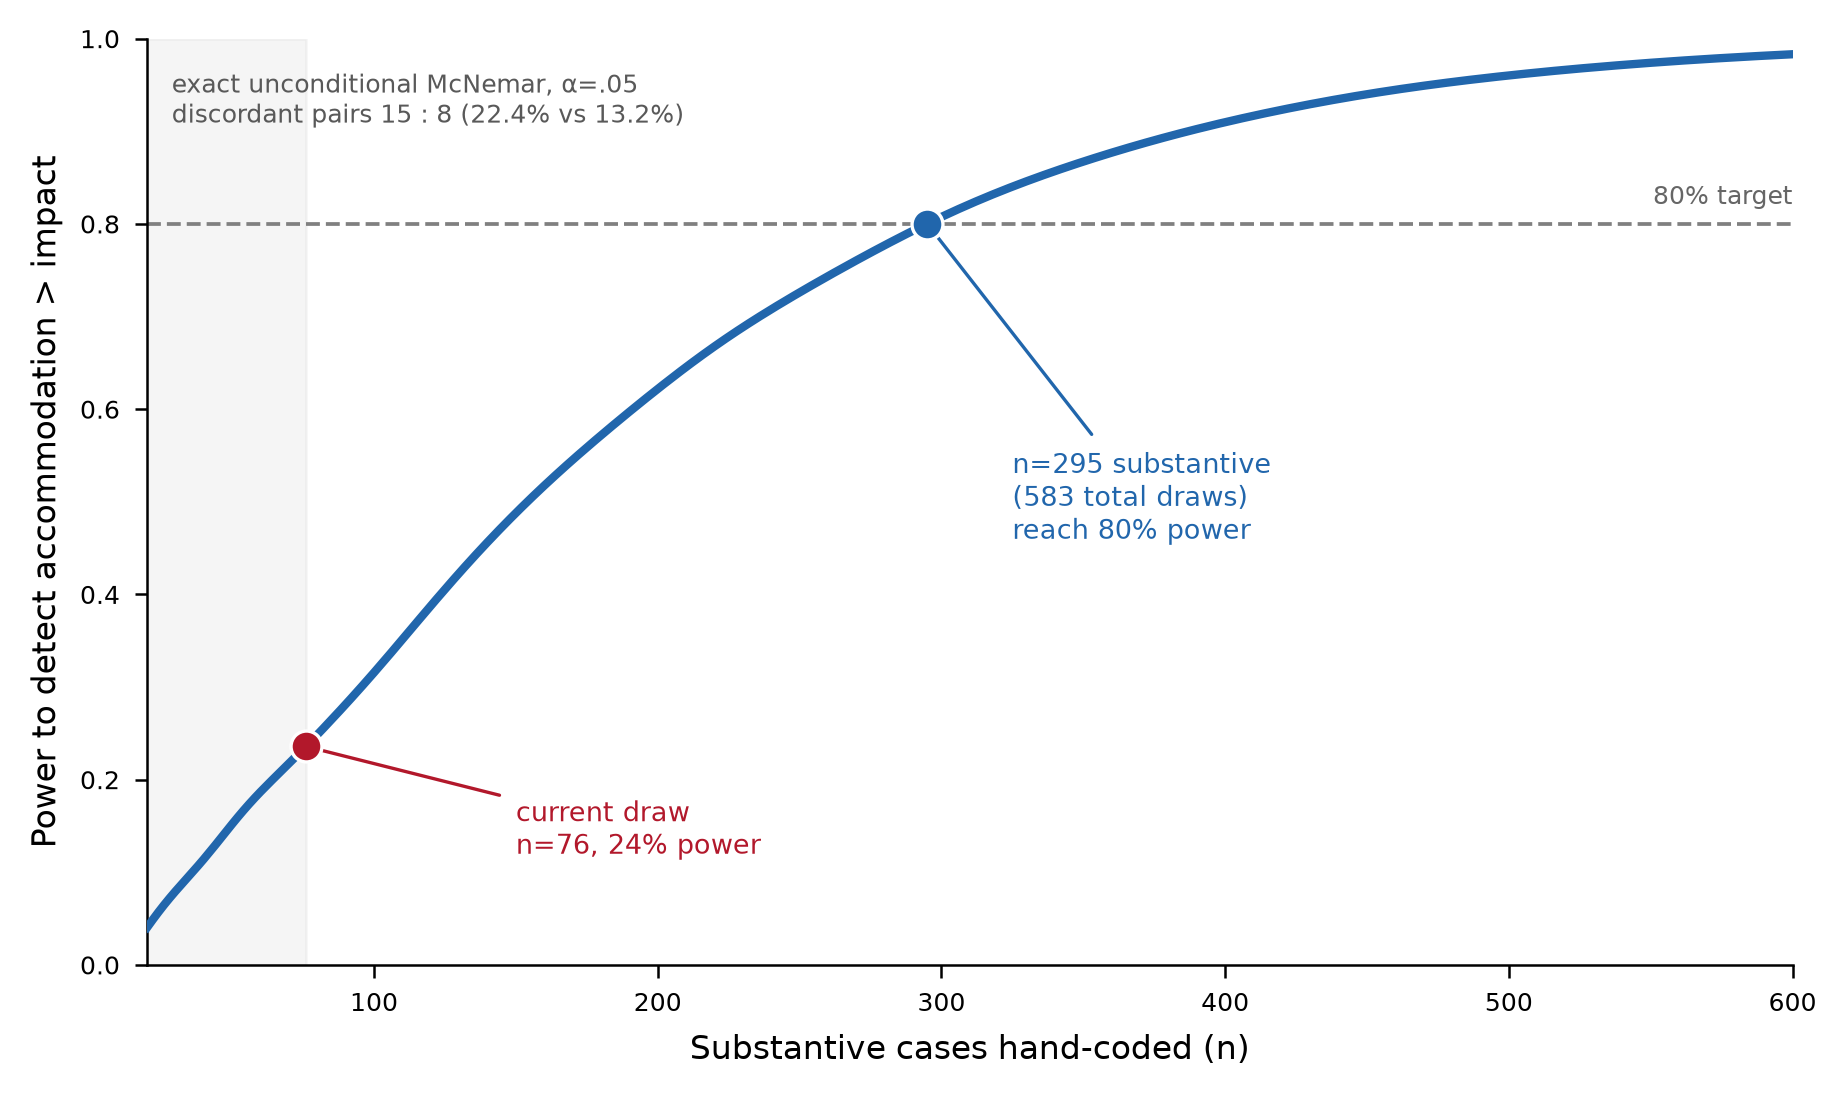
\includegraphics[width=\columnwidth]{media/image2.png}
\caption{The accommodation--impact gap needs roughly 300 substantive cases for nominal 80\% power.}
\label{fig:power}
\end{figure}

The trial-court result is a treatment lead with a method-sensitive accommodation estimate. The precision-recall correction gives 47.3\% treatment, 31.2\% accommodation, 12.5\% impact, 28.3\% refusal, and 9.4\% zoning. The LLM draw and the correction are two independent error models, a stronger extractor on a fresh random draw and a measurement-error correction of the rule system (Figure~\ref{fig:corrections}). They agree on treatment, impact, and zoning, which is evidence the treatment lead is not an artifact of either route.

\begin{figure}[H]
\centering
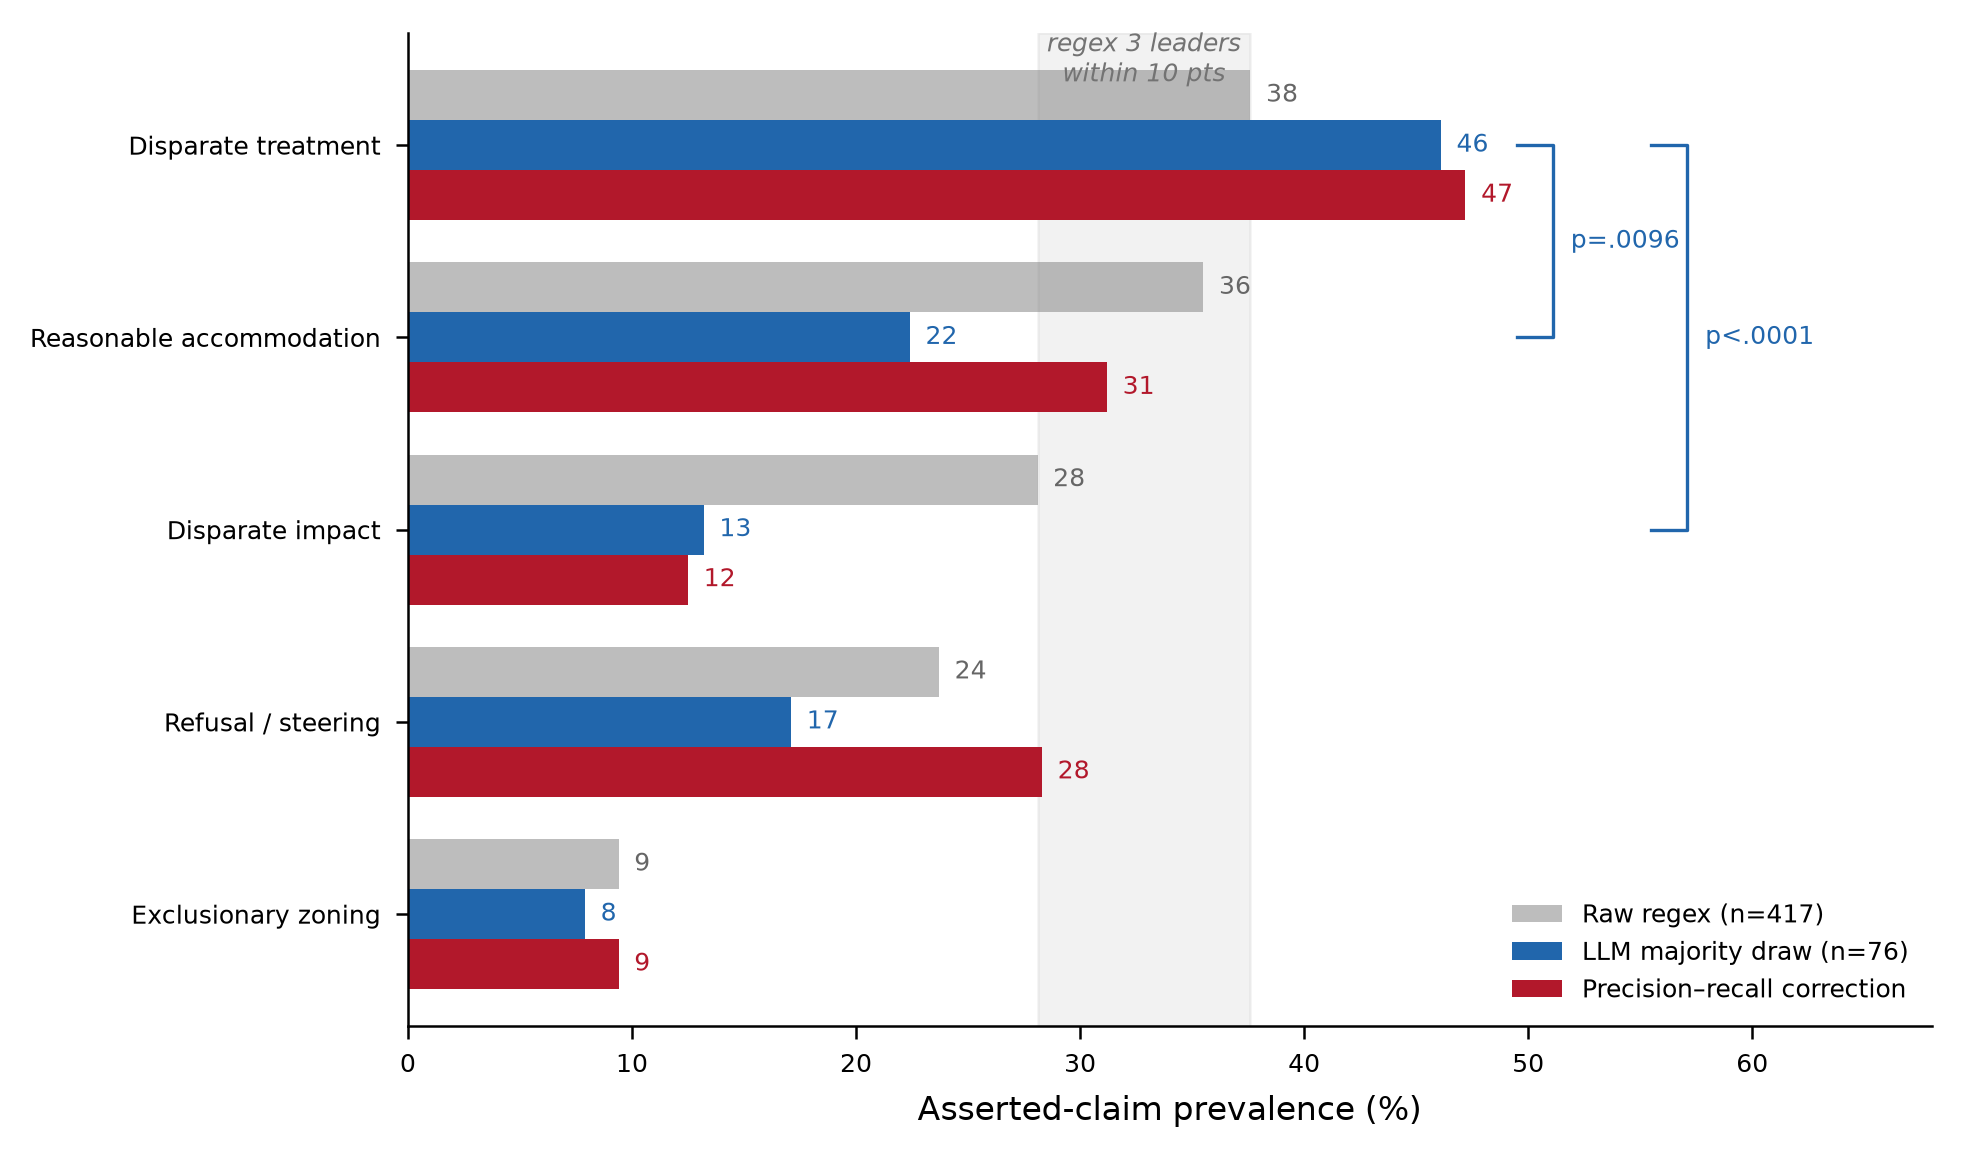
\includegraphics[width=\columnwidth]{media/image6.png}
\caption{Two independent corrections open a treatment lead over impact.}
\label{fig:corrections}
\end{figure}


Their divergence on accommodation and refusal marks where human coding would be most informative. Because the 93-case overlap is enriched and choice-based, corrected percentages are calibration scenarios. Shifting both overlap precision and recall by $\pm 0.10$, clipped to $[0,1]$, gives treatment 36.9--60.5\%, accommodation 25.9--39.1\%, impact 8.6--17.4\%, refusal 21.0--38.4\%, and zoning 7.3--12.1\%. These are sensitivity ranges, not confidence intervals. The appellate picture centered on disparate impact \citep{seicshnaydre2013} describes a different litigation stage. The district-court corpus provides a broader, treatment-centered account.

\subsection{A circuit split in doctrine}\label{sec:split}

Circuits diverge in the doctrine they apply. Disparate-impact language appears in 8\% of substantive clusters in the Tenth Circuit but 54\% in the Seventh, and disparate treatment ranges from 11\% to 61\%. The differences exceed sampling noise (impact $\chi^2=30.5$, $df=10$, $p=.0007$, Cram\'er's $V=0.27$; treatment $\chi^2=27.6$, $p=.0021$). The split echoes the appellate divergence \citet{seicshnaydre2013} documents. It also matters for the sorting question: the legal signal a household faces depends on which circuit governs, so the access channel is itself geographic. Per-circuit samples are small (18 to 67 clusters), so we read the split as a measured divergence, not a ranking of individual circuits.

Because circuits differ in claim mix, a raw enforcement ranking conflates doctrine with docket composition. Adjustment regresses the opinion-level strictness score $s_i$ on circuit indicators and the five claim labels, then reads each circuit off at the corpus-mean claim mix $\bar{y}_j$ rather than at its own:
\begin{align}
s_i &= \alpha + \gamma_{c(i)} + \sum\nolimits_j \beta_j\,\hat{y}_{ij} + \varepsilon_i,\label{eq:casemix}\\
\tilde{S}_c &= \alpha + \gamma_c + \sum\nolimits_j \beta_j\,\bar{y}_j.\label{eq:adjusted}
\end{align}
Because the circuit indicators force the within-circuit residuals to zero, the raw mean $\bar{S}_c$ exceeds $\tilde{S}_c$ by exactly $\sum_j \beta_j(\bar{y}_{jc} - \bar{y}_j)$, the circuit's departure from the average docket. That term is what a raw ranking reports as enforcement. Ranks on the two measures correlate at Spearman 0.14, and the ordering shifts under reweighting, so case-mix adjustment is a requirement rather than a refinement for any cross-circuit index. Appendix~\ref{app:feii} defines the components and plots the resulting circuit-year composite.

\subsection{Outcome cues}

Of 417 substantive clusters, 53 (12.7\%) contain a clear directional cue, and among those 53, 19 (35.8\%) are plaintiff-favorable, with Wilson 95\% interval $[24.3\%, 49.3\%]$. A directional phrase often omits the winning party, so the cue measures language, not a plaintiff-win rate. The sparsity of directional cues is itself a result, since most district opinions resolve on procedural or evidentiary grounds that leave no clean win--loss signal in text. Appendix~\ref{app:era} gives the era composition of asserted claims, which shifts toward accommodation over time.

\subsection{What the scoping model rules out}

The corpus cannot say whether the measured signal reaches housing, because the legal and housing series overlap in one year. A stylized Schelling sweep settles the narrower question of whether the channel is available at all, and the answer is conditional. Where the preference threshold is low, raising access lowers the mean same-type neighbour share from 0.778 to 0.723. At $\tau=.30$, many cross-group moves pass both gates but the final same-type share remains near 0.85; at $\tau=.45$, no cross-group move clears the preference rule. The preference rule therefore bounds what legal access can do, which makes the legal signal, the preference rule, and their interaction the three quantities a later identified design must measure together. This is a property of the model and not a finding about American housing. Appendix~\ref{app:scoping} gives the specification and the sweep.

\section{Discussion}

The trial-court docket differs from the appellate record, and this corpus measures that docket at scale. Two routes with different error models, a stronger extractor on a fresh draw and a measurement-error correction of the rule system, replace the near-flat regex ranking with a treatment lead.

Circuit rankings shift sharply once case mix is held constant (Figure~\ref{fig:casemix}), so an index that omits that adjustment reports docket composition as enforcement.

\begin{figure}[H]
\centering
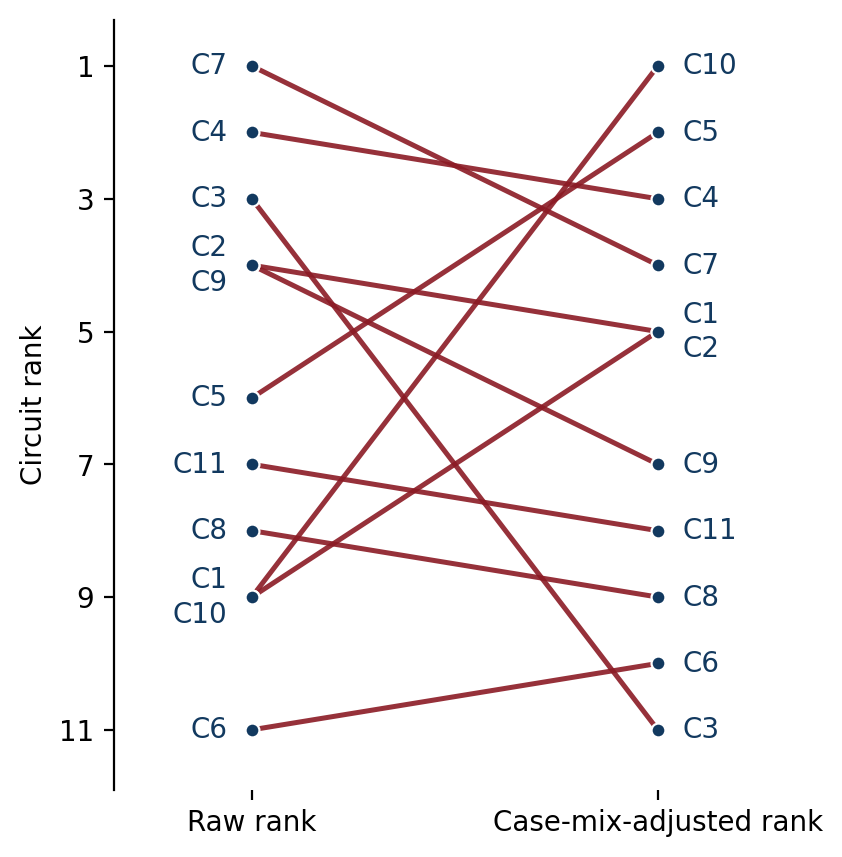
\includegraphics[width=0.58\columnwidth]{media/image7.png}
\caption{Circuit rankings shift sharply after case-mix adjustment.}
\label{fig:casemix}
\end{figure}

The released reasoning text gives a direct check on what varies most across these opinions. Clustering its TF--IDF and latent-semantic representation into three regimes yields groups whose distinguishing terms are procedural rather than doctrinal. The largest, 180 clusters, is characterised by \emph{complaint}, \emph{dismiss} and \emph{allegations}, the vocabulary of a Rule 12 posture; a second group of 116 turns on \emph{summary judgment}, \emph{genuine} and \emph{material fact}; the remaining 121 are docket-management orders marked by \emph{magistrate}, \emph{discovery} and \emph{objections}. None of the five constructs appears among the leading terms of any group. The first axis of variation in trial-court text is the stage at which a case was resolved, not the doctrine it applied, so an unsupervised summary of a docket recovers posture unless doctrine is measured directly.

A later design would measure legal exposure, the preference rule, and their interaction directly, using human coding of the random sample, non-overlapping housing outcomes, district-level legal units, and event studies around discrete circuit changes \citep{goodmanbacon2021,roth2022,sunabraham2021} with few-cluster inference \citep{cameron2008,mackinnon2018}.

Refusal or steering is the one construct where the stronger extractor does not help: $F_1$ falls from 0.667 to 0.607, and recall is 0.613 under the rule route and 0.548 under the model. Both therefore miss roughly two in five hand-coded positives, and a shortfall that sits in recall under both routes points at the construct rather than at either method. Opinions describe this conduct without a fixed vocabulary, as a unit already rented or a tour confined to one neighbourhood, so neither an enumerable lexicon nor a short codebook definition reaches it. We read that as an annotation problem before a modelling one.

The composition result bears on how the statute is read. The appellate literature is organized around disparate impact \citep{seicshnaydre2013}, while the trial docket measured here is led by disparate treatment at roughly three and a half times the impact share. The two are not in conflict. Appeals select for the claims worth appealing, and impact claims turn on contested legal standards that generate appellate opinions where treatment claims turn on facts that mostly do not. An account of the Act built from the appellate record therefore describes a selected tail, and trial-level composition has to be measured rather than inferred from it.

The outcome-cue result bounds what any index built on this text can carry. Only 53 of 417 substantive clusters, 12.7\%, contain a clear directional cue, and among those 35.8\% are plaintiff-favorable (Wilson 24.3--49.3\%). Most district opinions resolve on procedural or evidentiary grounds and leave no clean win--loss signal in the text. That sparsity is why the outcome-cue rate enters the enforcement index empirical-Bayes shrunk rather than raw: a circuit-year with two or three resolved cases would otherwise swing between 0 and 1 on a single phrase. It is also why the cue measures language rather than a plaintiff-win rate.

The recitation-versus-adjudication problem is not specific to this statute. Any doctrine with a canonical recitation invites the same rule-based error, and disparate impact is only a clean case of it because the three-step standard is quoted verbatim in opinions that decide nothing about impact. What a stored span gives a reader is the ability to locate such a match, not a guarantee that the match adjudicates. The exact model prompt, truncation implementation, raw responses, and evidence quotations are not in the release, so model inference itself is not reproduced. Results hold at their defined levels: 417 clusters for textual composition, 76 random-draw cases for the LLM comparison, 93 overlap cases for construct diagnostics, and eight one-year cells for feasibility.

\section{Conclusion}

FHA-443 makes the federal trial-level Fair Housing Act docket measurable. Rule-based extraction makes the three leading theories appear nearly tied; the frozen model labels put disparate treatment clearly first and cut disparate-impact false positives to zero. Circuits split from 8\% impact language to 54\%, so a cross-circuit index built on this text must be case-mix adjusted before it is read as enforcement.

For work that treats judicial text as a measurement instrument, a keyword rule and a codebook-driven model are not two accuracies of one measure but two different measures, and the distance between them is widest where a doctrine carries a canonical recitation.

Refusal and steering remain unsolved under both routes, at $F_1$ 0.67 and 0.61, the open problem this corpus hands to the next paper. The housing question we defer to a design able to measure exposure, preferences, and access together.

\section*{Limitations}

The corpus is a retrieval, not a census. It is district-only, CourtListener-derived, and selected by Nature of Suit coding and text availability, and litigated opinions are themselves a selected sample of disputes \citep{priest1984,seicshnaydre2013}. Every share describes this retrieval, and none should be transported to filings, settlements, or state-court practice.

The human overlap is enriched and choice-based, drawn to include machine-flagged holdings and a claim-by-era sample. That is the right design for finding extractor errors and the wrong one for estimating corpus-wide error rates, so Table~\ref{tab:gold} reports diagnostic rates. The corrected prevalences in Section~\ref{sec:docket} assume those rates transport, and shifting precision and recall by $\pm 0.10$ moves them materially.

The stronger extractor is one model at one setting, and 98.8\% unanimity across three passes says it is self-consistent rather than correct, though the Opus 5 replication in Section~\ref{sec:llm} shows the labels are not an artifact of that model choice. The 150-case draw carries model-generated labels, so it is a robustness comparison and not a gold standard. A human-coded random sample of 295 substantive cases would replace it and reach nominal 80\% power on the accommodation--impact gap, though the repository's assurance calculation shows even that size resolves the ordering with probability 0.64.

Refusal or steering is the weakest construct for both routes, at $F_1$ 0.67 and 0.61, and we cannot separate annotation difficulty from genuine heterogeneity in how courts describe the conduct. Per-circuit samples run from 18 to 67 clusters, so the split is a measured divergence and not a ranking of circuits.

The housing question that motivated the corpus stays open. Legal and housing coverage overlap in one year, yielding eight matched 2022 cells with no within-unit variation, so we report the merge as a feasibility result. The scoping model in Appendix~\ref{app:scoping} is stylized: a fixed grid, swept parameters, and no quantity estimated from the corpus. It states a condition; it measures nothing.

\section*{Ethics Statement}

The corpus consists of published federal court opinions, which are public records and carry no expectation of privacy. Party names appear in the source text as the courts published them. The release includes the frozen opinion text used by the offline pipeline, along with identifiers and derived labels; downstream users remain responsible for CourtListener's terms and any later source corrections.

The subject matter is litigation over protected characteristics, and the labels we release describe what a court discussed, not whether discrimination occurred. A positive disparate-treatment flag records that an opinion adjudicated a treatment theory. It does not record that a defendant discriminated, and it does not record that a plaintiff was wronged. We name this because an extractor of this kind is exactly the sort of artifact that gets reused as a scoreboard for jurisdictions, judges, or parties, and the measurement will not carry that weight. Per-circuit samples are as small as 18 clusters, outcome cues appear in 12.7\% of substantive opinions, and the directional cue records language rather than a plaintiff-win rate.

The intended use is descriptive research on trial-level doctrine and methodological work on legal information extraction. We discourage use in any individual case-level decision, in the evaluation of named judges, and in any application that treats a construct flag as a finding of liability.

\bibliography{refs}

\appendix


\section{Pipeline protocol}\label{app:protocol}

The pipeline measures Fair Housing Act legal signals from federal district-court opinion text and aggregates them by circuit geography. The canonical snapshot holds 757 NOS-443 opinion clusters, 751 with full text, and 417 rule-positive substantive clusters.

Three analytic scales apply. The opinion cluster, one district-court decision, is the measurement unit, and clusters can share a docket rather than mapping to filings. Circuit geography aggregates the 11 numbered circuits, none in the District of Columbia. The housing feasibility cell is a circuit-vintage merge with eight substantive matches, all in 2022. No appellate corpus or circuit-court doctrine is claimed. Per-opinion variables store snippets and character offsets, with the outcome cue null when cues are mixed or absent. Legal-signal breadth is a descriptive output, not an index component.

One deterministic forward pass begins from the hash-verified full-text snapshot: identify substantive FHA by the rule of Equation~\ref{eq:inclusion}; extract variables with evidence spans; aggregate the enforcement index; merge housing feasibility inputs; check estimability, recording an insufficient-panel note and fitting no real-data panel model; run validation diagnostics; rescore the frozen LLM labels; sweep the gatekeeping scenarios on a seeded grid; and regenerate the figures and claim audit. Stochasticity is seeded throughout. The claim builder reads the written outputs, emits machine-readable audit tables, and checks every declared headline value, exiting non-zero on an unchecked or disagreeing claim. A released breadth score,
\begin{equation}\label{eq:breadth}
\begin{split}
s = \min\big(1,\; & .35\,\mathrm{DI} + .25\,\mathrm{HUD} + .20\,\mathrm{RA}\\
                  & + .10\,\mathrm{prec} + .10\,\mathrm{fw}\big)
\end{split}
\end{equation}
is descriptive only and enters no composite. Table~\ref{tab:params} lists the parameters frozen across the pass.

\begin{table}[h]
\centering\small
\setlength{\tabcolsep}{3pt}
\begin{tabular}{ll}
\toprule
Parameter & Value \\
\midrule
Grid / vacancy / groups & $20\times20$ Moore / 10\% / 2 \\
$\tau$ / access / seed & $\{.20,.30,.45\}$ / 5 / fixed \\
Min text length / NOS filter & 200 chars / canonical 443 \\
ACS vintages & 2012, 2017, 2022 \\
Housing merge & 8 cells; one year; no TWFE \\
\bottomrule
\end{tabular}
\caption{Frozen parameters.}
\label{tab:params}
\end{table}

\section{The enforcement index}\label{app:feii}

The Federal Enforcement Intensity Index for circuit $c$ in year $t$ is
\begin{equation}\label{eq:feii}
\mathrm{FEII}_{ct} = \tfrac{1}{3}\left[z(\log(1+n_{ct})) + z(S_{ct}) + z(R_{ct})\right]
\end{equation}
where $n_{ct}$ is opinion volume, $S_{ct}$ the directional outcome-cue rate, and $R_{ct}$ mean remedy-cue intensity,
\begin{equation}\label{eq:remedy}
R_{ct} = \frac{1}{n_{ct}}\sum_i r_i .
\end{equation}
Equivalently, $\mathrm{FEII}_{ct} = \sum_k w_k\, z(X^k_{ct})$ over the three components with $w_k = \tfrac{1}{3}$. We weight equally because no external enforcement label exists against which to fit weights; a data-driven weighting would encode an unsupported ranking, and the released components let a user reweight or drop a channel. The outcome-cue rate is empirical-Bayes shrunk with pseudo-count $k=4$, since a circuit-year holding two or three resolved cases would otherwise swing between 0 and 1. Component values by circuit are shown in Figure~\ref{fig:feii}; a circuit high on opinion volume need not rank high on remedy-cue intensity or outcome direction.

\begin{figure}[H]
\centering
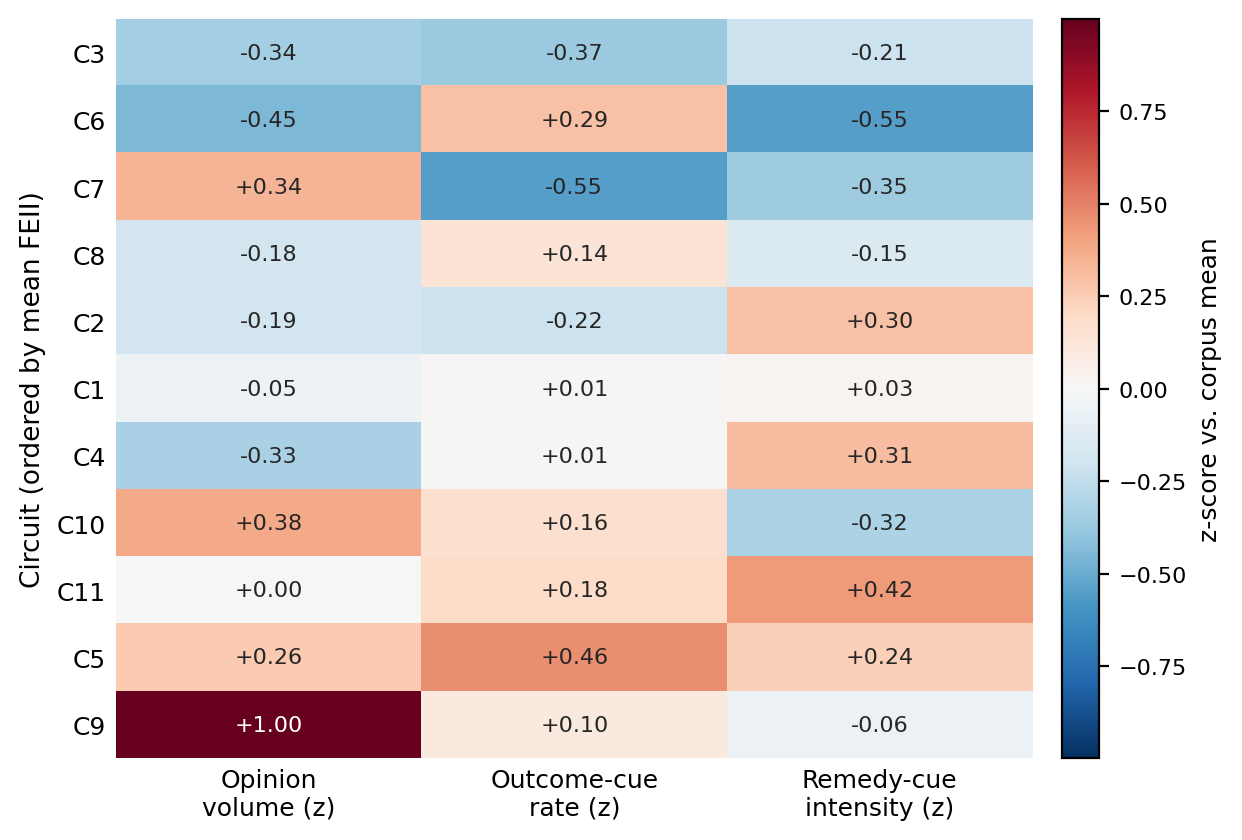
\includegraphics[width=\columnwidth]{media/image4.png}
\caption{Circuit enforcement-index components as standardized deviations.}
\label{fig:feii}
\end{figure}

\section{The scoping model}\label{app:scoping}

The model initializes a $20\times20$ Moore-neighborhood grid with two equally sized groups and 10\% vacancies. An agent accepts a vacant cell only when its same-type neighbor share, excluding the focal household, meets a preference threshold $\tau$. Unsatisfied agents and a 4\% turnover draw seek new cells, and a separate gatekeeping rule can block a cross-group move that otherwise meets $\tau$ (Figure~\ref{fig:gates}). Writing $\pi$ for the probability that such a move is denied, $g$ for barrier strength and $e$ for the access parameter,
\begin{equation}\label{eq:access}
\begin{gathered}
\pi = g\,(1-e),\quad g = .80,\\
e \in \{.15,.325,.50,.675,.85\}
\end{gathered}
\end{equation}
We sweep $\tau$ and the access parameter $e$ independently and run 250 update cycles and 40 replications per cell with a fixed seed. The observed circuit-mean FEII span is recorded as reference metadata only; no mapping from FEII to $e$ is estimated. Because denial probability is $g(1-e)$, $e$ is a monotone access parameter rather than the realized admission probability.

\begin{figure}[H]
\centering
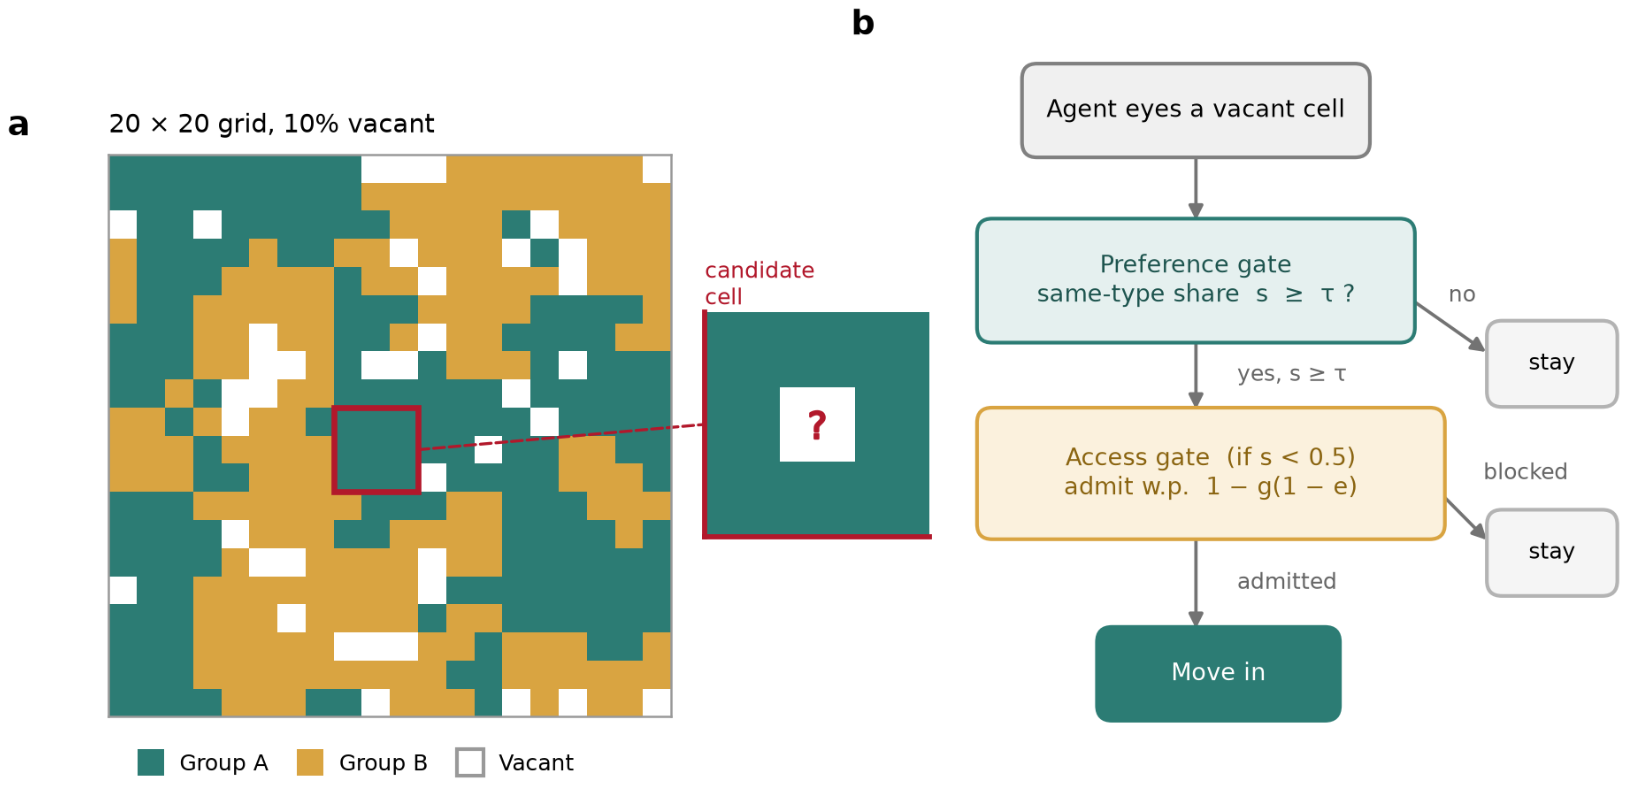
\includegraphics[width=\columnwidth]{media/image18.png}
\caption{Two sequential gates: a preference threshold $\tau$, then a cross-group access barrier. Swept values are $\tau \in \{0.20, 0.30, 0.45\}$ for the preference threshold and five access levels $e$, with barrier strength $g = 0.80$.}
\label{fig:gates}
\end{figure}

At $\tau=0.20$, the mean same-type neighbor share falls from 0.778 at access 0.15 to 0.723 at 0.85. At $\tau=0.30$ it stays near 0.85, and at $\tau=0.45$ no cross-group move clears the threshold while the share stays near 0.92 (Figure~\ref{fig:surface}). The asymmetry is a property of the model, not a finding about American housing: access moves sorting only where the preference rule permits cross-group moves, so the preference rule bounds the effect legal access can have.

\begin{figure}[H]
\centering
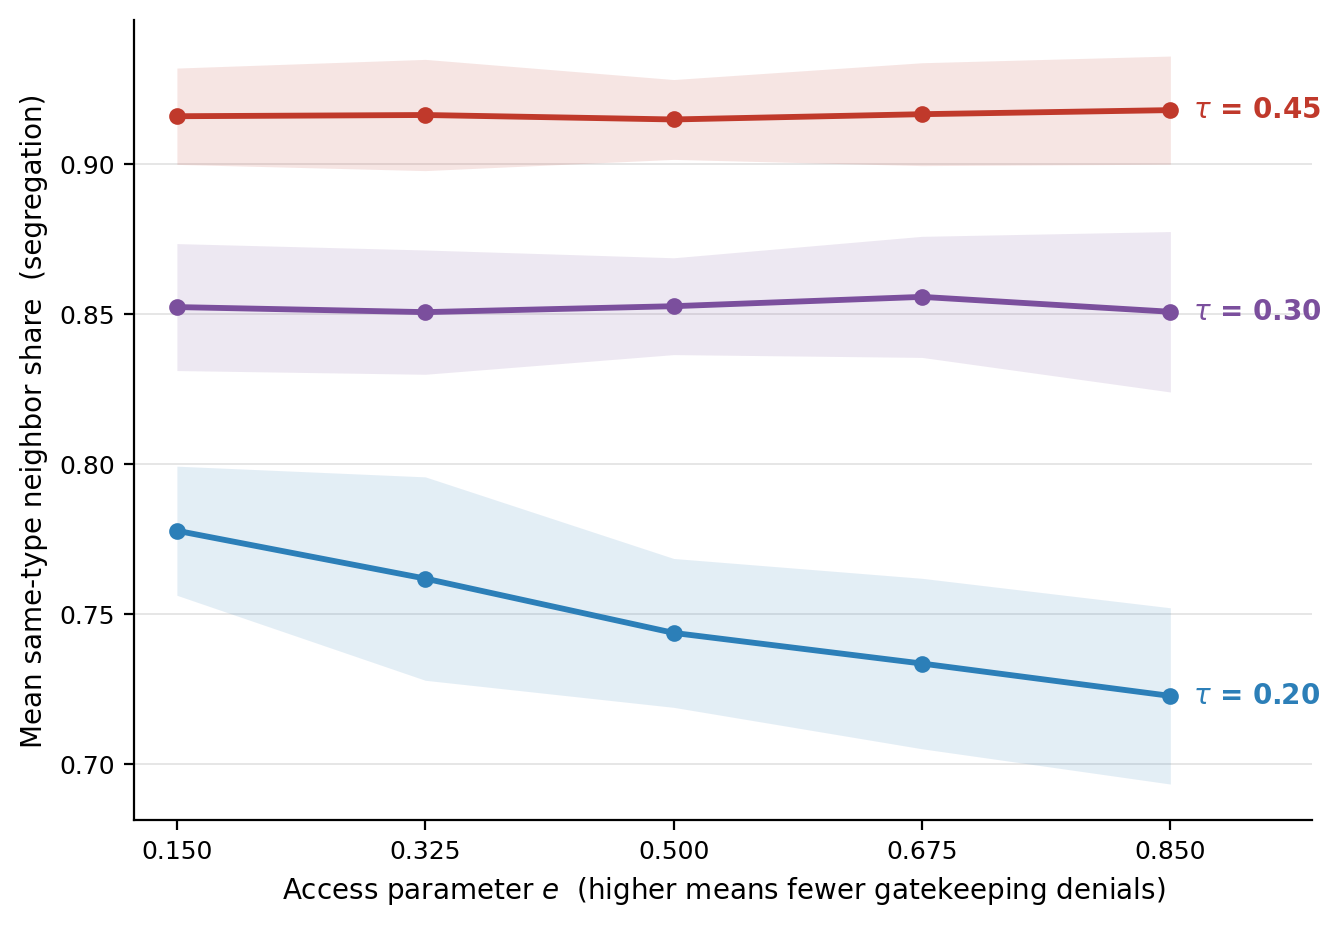
\includegraphics[width=\columnwidth]{media/image3.png}
\caption{Access lowers segregation only when preference thresholds stay low.}
\label{fig:surface}
\end{figure}

\section{Negation-scoping sensitivity}\label{app:negation}

The extraction rules match a construct wherever its lexicon fires, including inside a negated clause. Table~\ref{tab:negation} reports what each headline indicator does when the negation-sensitive variant replaces the unscoped rule used in the headline run. Every shift is zero or negative, because scoping can only withdraw a flag, and the largest is disparate treatment at 2.40 points. No construct changes rank, so we report the unscoped rule and this table rather than switching: the choice is visible and it does not carry the result.

\begin{table}[!ht]
\centering\small
\begin{tabular}{lr}
\toprule
\textbf{Indicator} & \textbf{Change (pp)} \\
\midrule
Outcome-cue rate & $+0.00$ \\
Refusal / steering & $+0.00$ \\
Zoning / exclusionary & $-0.24$ \\
Disparate impact & $-0.48$ \\
Legal-signal breadth & $-0.58$ \\
Reasonable accommodation & $-0.96$ \\
Disparate treatment & $-2.40$ \\
\bottomrule
\end{tabular}
\caption{Negation-scoping sensitivity of headline indicators.}
\label{tab:negation}
\end{table}

\section{Claim composition by era}\label{app:era}

Figure~\ref{fig:era} splits the substantive clusters into three periods and plots the share of opinions asserting each construct. Reasonable accommodation rises across the three periods while disparate impact, refusal or steering, and exclusionary zoning fall. The era boundaries are calendar cuts rather than doctrinal events, and the per-era samples are small, so the figure describes how the composition of this retrieval moves over time and not a trend in filing or in judicial behaviour.

\begin{figure}[H]
\centering
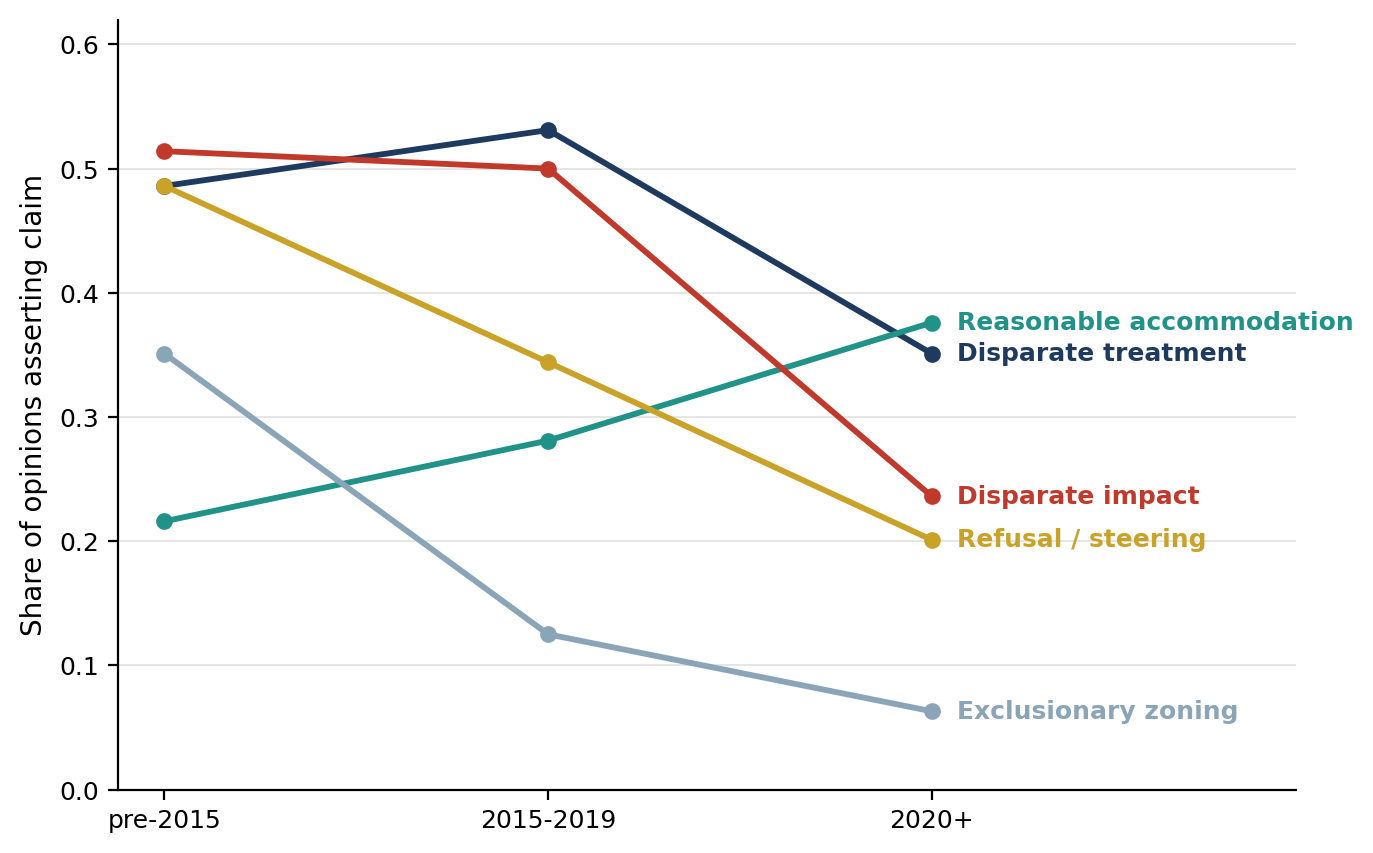
\includegraphics[width=\columnwidth]{media/image12.png}
\caption{Claim composition shifts toward accommodation across eras.}
\label{fig:era}
\end{figure}

\section{Pipeline diagram}\label{app:pipeline}

Figure~\ref{fig:pipeline} condenses the nine stages of Appendix~\ref{app:protocol} into a single forward pass, with edge labels naming the section that produces each object. The blind gold set enters at validation only, so no hand-coded label reaches the extraction rules.

\begin{figure}[H]
\centering
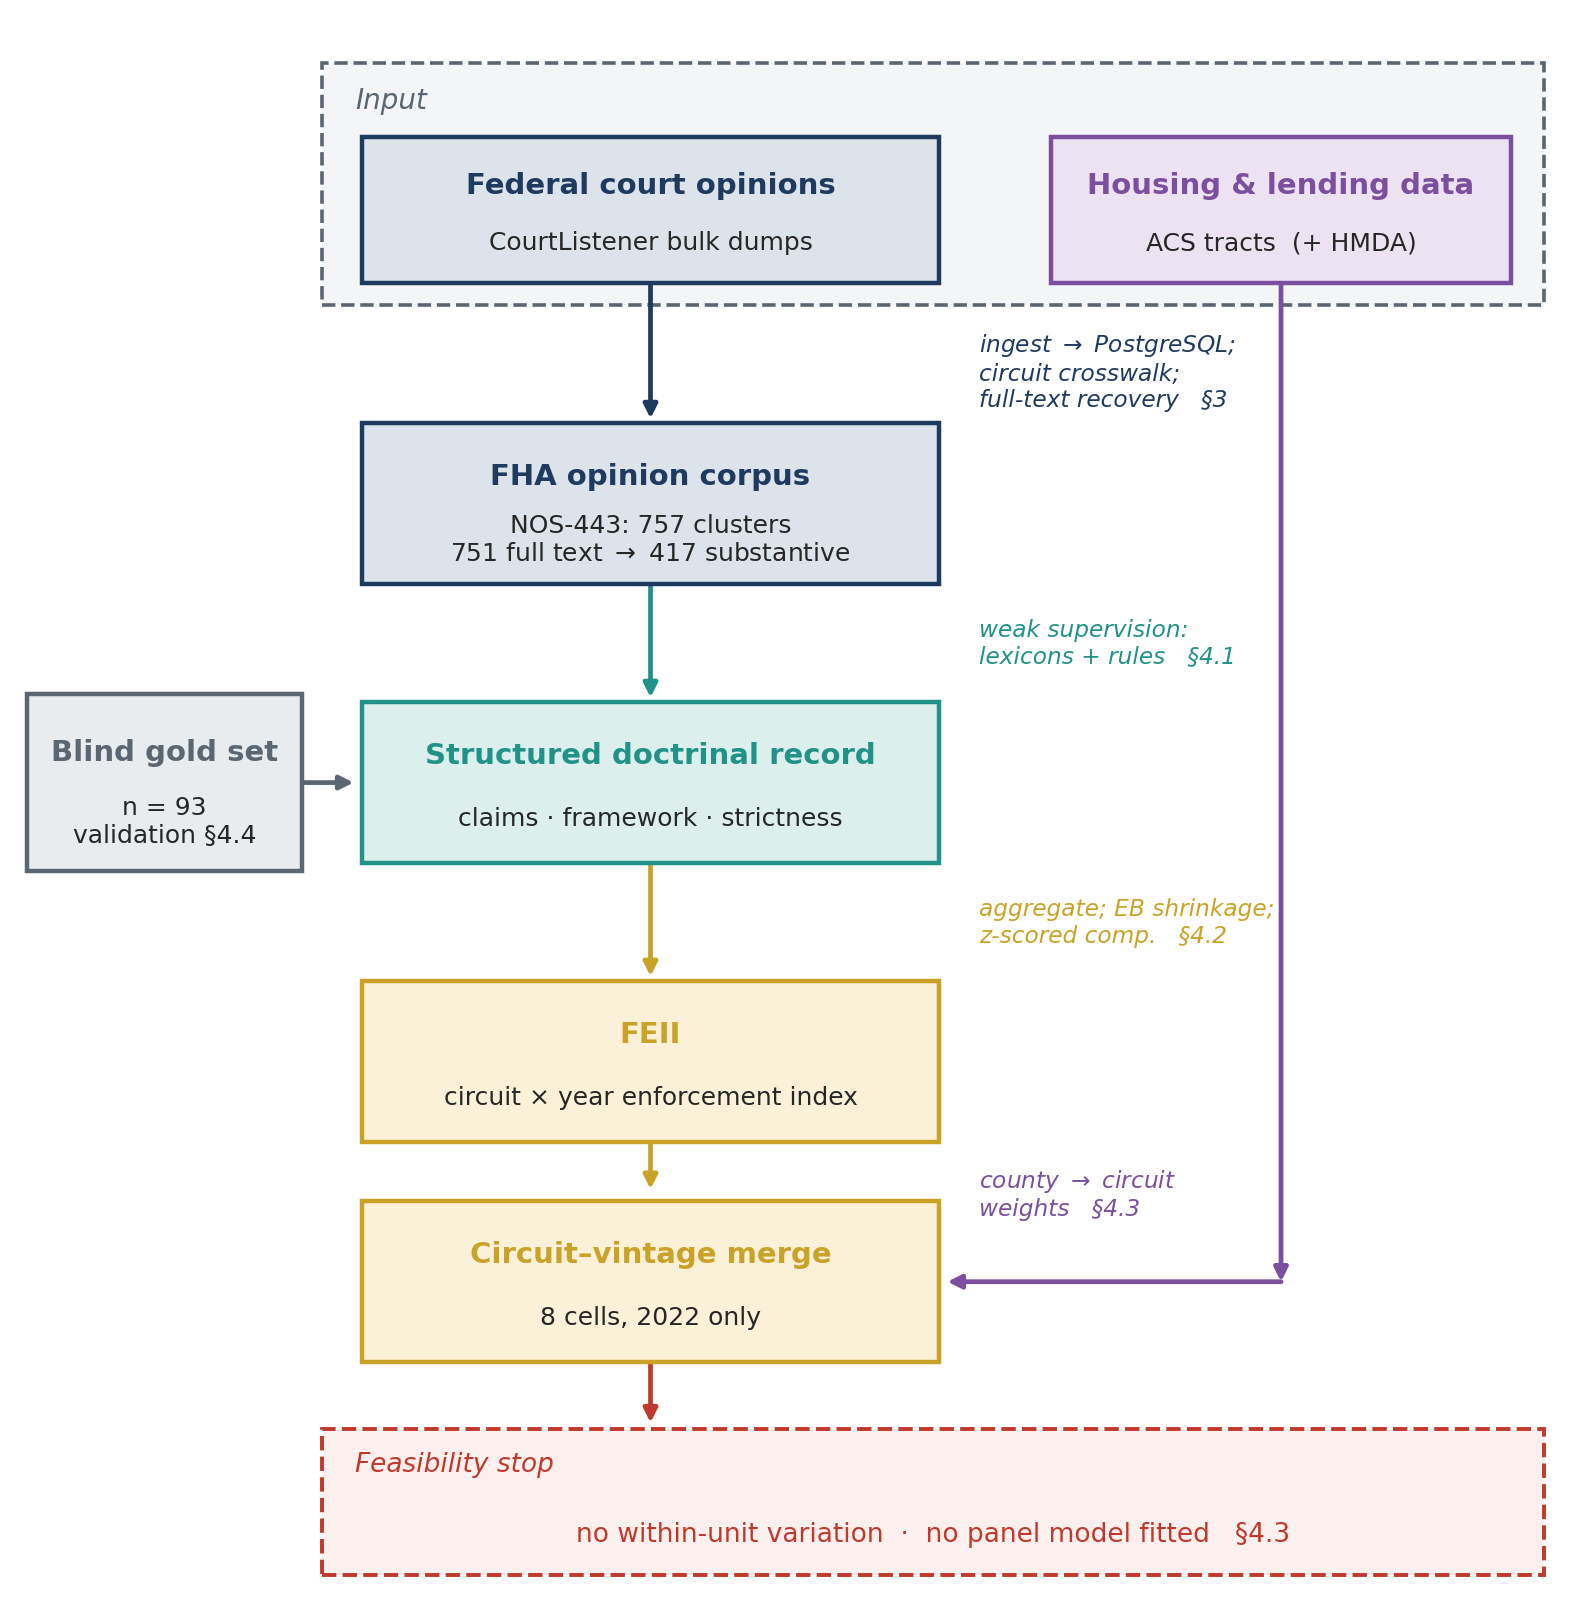
\includegraphics[width=0.9\columnwidth]{media/image9.png}
\caption{FHA measurement and feasibility pipeline.}
\label{fig:pipeline}
\end{figure}

\section{Annotation codebook}\label{app:codebook}

The released codebook gives the instructions used for human coding and supplied to the LLM baseline. The core rule is scoping: code what the opinion itself adjudicates or substantively discusses as an asserted FHA theory, and never code a claim because a phrase appears in a string-cited case name, a quoted statute, or procedural history. The instructions require a short verbatim quote for every positive label, but the released human and model label files retain classifications rather than claim-level quotations; those quotations therefore cannot be audited from the frozen outputs.

The five claim labels are binary and not mutually exclusive. \emph{Disparate treatment} is intentional discrimination because of a protected characteristic: differential terms or treatment, pretext analysis, or discriminatory animus, often though not always analyzed under McDonnell Douglas. \emph{Disparate impact} is a facially neutral policy challenged for its discriminatory effect and requires effects-based reasoning such as statistics, robust causality, or the HUD three-step framework; the codebook forbids coding it from a citation, a legal-standard recitation, or a claim the court declines to reach, which is exactly the failure mode Section~\ref{sec:validation} measures in the regex route. \emph{Refusal or steering} covers refusal to rent, sell, or negotiate, steering, and misrepresented availability under \S~3604(a) and (d). \emph{Reasonable accommodation} is the disability-based duty of \S~3604(f)(3)(A)--(B), including failure-to-accommodate and interactive-process disputes. \emph{Exclusionary zoning} covers municipal land use, permitting, occupancy limits, and siting decisions challenged as discriminatory.

The framework label takes exactly one of four values: \texttt{mcdonnell} when McDonnell Douglas burden shifting is explicitly applied, \texttt{hud} when the HUD or Inclusive Communities framework is, \texttt{both}, or \texttt{none}.

\section{Frozen LLM baseline protocol}\label{app:llmprotocol}

The LLM comparison is a frozen artifact, and reproduction makes no model call. Three independent passes of Claude Opus 4.8 labeled each opinion under the Appendix~\ref{app:codebook} codebook, and the per-field majority vote is the reported label. Of 729 requested passes, 728 returned; the missing pass is cluster 9672005, whose two returned passes agree on every field. The 93-case human overlap is the only set scored against a reference label. The 150-case random draw, seed 20260720 from the 658-case non-overlap frame, carries model silver labels and supports only the robustness and prevalence analyses.

The open-weight comparison in Section~\ref{sec:llm} relabels the same 93 opinions with qwen3:32b at four-bit quantization, served through Ollama on two T4 GPUs under a 32{,}768-token window that admits every opinion whole. Decoding is greedy, so repeated passes are byte-identical on 389 of 390 cells and the majority vote of Equation~\ref{eq:vote} collapses to a single pass. Model family, parameter count, quantization, and serving stack all differ from the frozen baseline at once, so the recall gap is not attributable to open weights alone; the precision comparison, which is the claim made in Section~\ref{sec:llm}, does not depend on separating them. Per-opinion labels are released alongside the frozen artifact.

The release commits all three per-pass label sets, the majority votes, the sample index, and the codebook. Recomputation is asserted rather than assumed: the scoring script rebuilds the majority votes from the per-pass labels and fails if the committed file disagrees, and the draw script verifies the committed sample index against the seed.

\section{Circuit-level construct shares}\label{app:circuit}

Table~\ref{tab:circuits} reports the raw regex share of each construct by circuit, the basis of the divergence statistics in Section~\ref{sec:split}. These are uncorrected rule-based shares on the 417 substantive clusters, so the disparate-impact column inherits the 0.41 precision documented in Section~\ref{sec:validation} and overstates impact everywhere; the cross-circuit ordering, not the level, is the quantity of interest. Per-circuit samples run from 18 clusters in the First to 67 in the Second, and the extremes of the impact column, 7.9\% in the Tenth against 53.7\% in the Seventh, are the split quoted in the abstract.

\begin{table}[h]
\centering\small
\setlength{\tabcolsep}{4pt}
\begin{tabular}{rrrrrrr}
\toprule
Cir. & $n$ & Treat. & Impact & Refusal & Accom. & Zoning \\
\midrule
1 & 18 & .278 & .167 & .167 & .333 & .056 \\
2 & 67 & .463 & .373 & .224 & .179 & .149 \\
3 & 27 & .444 & .333 & .370 & .481 & .222 \\
4 & 30 & .500 & .333 & .300 & .300 & .033 \\
5 & 45 & .311 & .244 & .244 & .378 & .067 \\
6 & 28 & .107 & .143 & .250 & .250 & .000 \\
7 & 41 & .610 & .537 & .317 & .366 & .122 \\
8 & 23 & .391 & .174 & .130 & .435 & .130 \\
9 & 61 & .344 & .279 & .213 & .443 & .033 \\
10 & 38 & .316 & .079 & .132 & .421 & .105 \\
11 & 39 & .256 & .231 & .256 & .410 & .103 \\
\bottomrule
\end{tabular}
\caption{Raw regex construct shares by circuit on the 417 substantive clusters. Uncorrected; see Section~\ref{sec:validation} for construct-level precision.}
\label{tab:circuits}
\end{table}

\section{Second-pass agreement}\label{app:secondpass}

A 30-case second pass by an independent coder, blind to both the first pass and machine output, measures the stability of the human reference itself. Claim-level agreement is 95.3\% ($\kappa=0.899$), framework agreement 93.3\% ($\kappa=0.864$), and four-way outcome agreement 80.0\% ($\kappa=0.726$); on the 16 cases where both coders saw a decisive binary outcome, agreement is exact. The construct diagnostics in Table~\ref{tab:gold} therefore sit well inside the reliability of the labels they are scored against, and the weakest agreement, on the four-way outcome, matches the paper's decision to report directional outcome cues descriptively rather than build on them.

\end{document}
